%% simp-gps.tex,  version 22/04/17

%%%%%%%%%%%%%%%%%%%%%%%%%%%%%%%%%%%%%%%%%%%%%%%%
\section{Simplicial Groups} \label{sect:simpgps}

This material is taken mainly from seminars given by Tim Porter, 
designed to explain the four functors in the diagram
$$
\xymatrix{
\text{Spaces} \ar[rr]<-1.0ex>_{\Sing}
  && \text{Simplicial Sets} \ar[rr]<-1.0ex>_{G} \ar[ll]<-1.0ex>_{|~|}
     && \text{Simplicial Groupoids} \ar[ll]<-1.0ex>_{W}
}
$$

\bigskip
\subsection{Simplicial Sets and Simplicial Complexes} \label{subsect:simpsets}

A \emph{simplicial set} $S$ comprises 
\begin{itemize}
\item 
a sequence $\{S_n\}_{n \geqslant 0}$ of sets, 
where $S_n$ is the \emph{set of simplices of dimension $n$}, linked by 
\item 
\emph{face maps} $d_k : S_n \to S_{n-1}, 0 \leqslant k \leqslant n$, 
where we think of $d_k(S_n)$ as the ``face opposite $S_n$'', and 
\item
\emph{degeneracy maps} $s_k : S_n \to S_{n+1}, 0 \leqslant k \leqslant n$. 
\end{itemize} 

\noindent
A \emph{simplicial complex} $K$ is a set $V(K)$ of vertices, and a family  
$S \subset \left( 2^{V(K)}_{{\rm fin}} \setminus\emptyset \right)$ 
closed under $\subseteq$. 

\noindent
To get from a simplicial complex $K$ to a simplicial set $S_K$
\begin{itemize}
\item
pick a total order on $V(K)$, 
\item 
let $S_K$ be the set of all finite subsets of $V(K)$, 
\item 
set $(S_K)_n = \{ [a_0,\ldots,a_n] ~|~ \{a_0,\ldots,a_n\} \in S, 
                                       a_0 \leqslant \cdots \leqslant a_n \}$.
\item
choose face maps $d_i[a_0,\ldots,a_n] = [a_0,\ldots,\hat{a_i},\ldots,a_n]$, 
omitting the $i$-th entry, starting at $0$, 
\item
choose degeneracy maps 
$s_i[a_0,\ldots,a_n] = [a_0,\ldots,a_i,a_i,\ldots,a_n]$, 
duplicating the $i$-th entry.
\end{itemize}

\begin{example}
\emph{Here is a simplicial complex $K$ with $4$ vertices; $4$ edges; 
and $1$ triangle.} 
\begin{center}
\includegraphics[scale = 0.7]{simp-gps/simp-set.eps}
%% \input{simp-set.pstex_t}
\end{center}
\begin{eqnarray*}
   V(K) &=& \{0,1,2,3\}, \\
      S &=& \{~ \{0,1,2\},~ \{2,3\},~ \{0,1\},~ \{1,2\},~ \{0,2\},~ 
             \{0\},~ \{1\},~ \{2\},~ \{3\}~ \} \\
\text{\emph{order}} &=& 2 < 1 < 3 < 0 \quad\text{\emph{(say)}},\\
(S_K)_0 &=& \{ [2],~ [1],~ [3],~ [0] \}, \\
(S_K)_1 &=& \{ [2,2]=s_0[2],~ [1,1]=s_0[1],~ [3,3]=s_0[3],~ [0,0]=s_0[0],~ 
                       [2,1],~ [2,3],~ [2,0],~ [1,0] \}, \\
(S_K)_2 &=& \{ [2,2,2]=s_0^2[2],~ [1,1,1]=s_0^2[1],~ [3,3,3]=s_0^2[3],~ 
               [0,0,0]=s_0^2[0],~ [2,2,1]=s_0[2,1],~ \\
        & &  \qquad  [2,2,3]=s_0[2,3],~ [2,2,0]=s_0[2,0],~ [2,1,1]=s_1[2,1],~ 
               [2,3,3]=s_1[2,3],~ \\ 
        & &  \qquad  [2,0,0]=s_1[2,0],~ [1,1,0]=s_0[1,0],~ [1,0,0]=s_1[1,0],~ 
               [2,1,0] \}. 
\end{eqnarray*}
\end{example}

\noindent
The face and degeneracy maps satisfy the following identities.
~{\bf [need to check these!]}  \\
The second column gives the common image of $[a_0,\ldots,a_n]$.
\begin{equation} \label{eq:face-degen} 
\begin{tabular}{ll}
$d_{j-1} \circ d_i ~=~ d_i \circ d_j\quad (0 \leqslant i < j \leqslant n)$ 
  & $\quad[a_0,\ldots,\hat{a_i},\ldots,\hat{a_j},\ldots,a_n]$, \\
$d_{j+1} \circ s_i ~=~ s_i \circ d_j\quad (0 \leqslant i < j \leqslant n)$ 
  & $\quad[a_0,\ldots,a_i,a_i,\ldots,\hat{a_j},\ldots,a_n]$, \\
$d_{i+1} \circ s_i ~=~ d_i \circ s_i ~=~ \id
\quad (0 \leqslant i \leqslant n)$ 
  & $\quad[a_0,\ldots,a_n]$, \\
$d_i \circ s_j ~=~ s_{j-1} \circ \quad (0 \leqslant i < j \leqslant n)$ 
  & $\quad[a_0,\ldots,\hat{a_i},\ldots,a_j,a_j,\ldots,a_n]$, \\
$s_{j+1} \circ s_i ~=~ s_i \circ s_j\quad (0 \leqslant i < j \leqslant n)$ 
  & $\quad[a_0,\ldots,a_i,a_i,\ldots,a_j,a_j,\ldots,a_n]$, \\
$s_{i+1} \circ s_i ~=~ s_i^2 \qquad\qquad (0 \leqslant i \leqslant n)$ 
  & $\quad[a_0,\ldots,a_i,a_i,a_i,\ldots,a_n]$. \\
\end{tabular}
\end{equation}

\bigskip\noindent
%%%%%%%%%%%%%%%%%%%%%%%%%%%%%%%%%%%%%%%%%%
{\bf The standard $n$-simplex, $\Delta^n$} 

\medskip\noindent
(See Ehlers \cite{ehlers} for some of this material.)

Let $B_{n+1} = \{\bsye_0,\ldots,\bsye_n\}$ be the standard basis for 
$\bbR^{n+1}$, and let $\Delta^n$ be the convex hull of the points $B_{n+1}$, 
a subset of the hyperplane $x_0 + x_1 + \cdots + x_n = 1$. 
The picture below shows $\Delta^2 \subseteq \bbR^3$.
\begin{center}
\includegraphics[scale = 0.7]{simp-gps/n-simplex.eps}
%% \input{n-simplex.pstex_t} 
\end{center}
Any $\bsyx \in \Delta^n$ may be expressed as 
$$
\bsyx ~=~ \sum_{i=0}^n\; x_i\,\bsye_i, \qquad 
\sum_{i=0}^n\;x_i ~=~ 0, \qquad x_i \geqslant 0.
$$
We then define the \emph{linear} maps 
$$
\delta_k ~:~ \Delta^{n-1} \to \Delta^n, \qquad 
(x_0,\ldots,x_{n-1}) \mapsto (x_0,\ldots,x_k,0,x_{k+1},\ldots,x_{n-1}), 
%% \bsye_i \mapsto \left\{ 
%% \begin{array}{ll} \bsye_i & (i < k), \\
%%                   \bsye_{i+1} & (i \geqslant k), 
%% \end{array} \right.
\qquad 0 \leqslant k \leqslant n. 
$$
Similarly, we define 
$$
\sigma_k ~:~ \Delta^n \to \Delta^{n-1}, \qquad 
(x_0,\ldots,x_n) \mapsto (x_0,\ldots,x_{k-1},x_k+x_{k+1},x_{k+2},\ldots,x_n), 
\qquad 0 \leqslant k \leqslant n-1. 
$$ 
The picture for $\Delta^2$ is 
\begin{center}
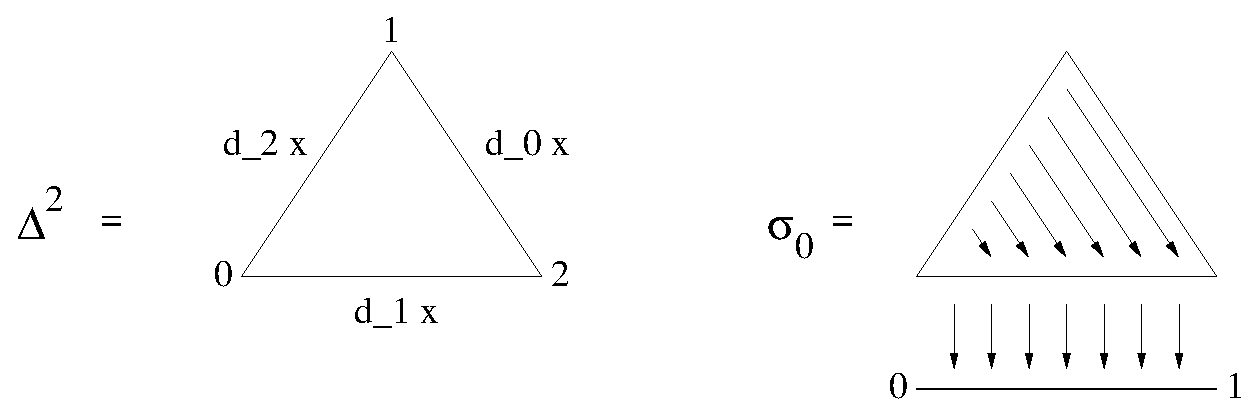
\includegraphics[scale = 0.7]{simp-gps/n-sigma.eps}
%% \input{n-sigma.pstex_t} 
\end{center}


\newpage\noindent
%%%%%%%%%%%%%%%%%%%%%%%%%%%%%%%%%%%%%%%%%%%%%%%%%%%%%
{\bf The Singular Complex $\Sing(X)$ of a space $X$.}

\medskip
For $X$ a space we defing the \emph{singular complex} of $X$ to be 
the set of maps 
$$
\Sing(X) ~=~ \Top(\Delta^n,X). 
$$

The diagram below shows such a map $\tau$ to a space $X$ with two holes.
\begin{center}
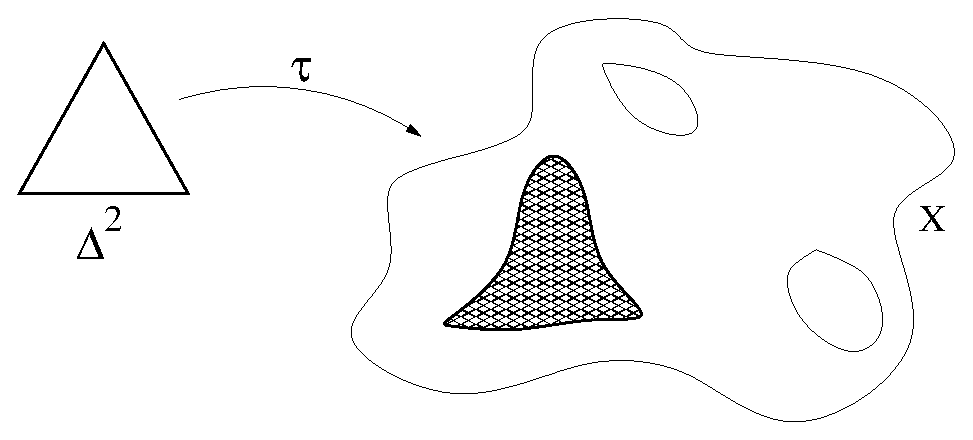
\includegraphics[scale = 0.7]{simp-gps/delta2X.eps}
%% \input{delta2X.pstex_t} 
\end{center}


\bigskip\noindent
{\bf The Nerve of a Category} 

\medskip/noindent
Let $\bbC$ be a small category. 
The \emph{nerve} of $\bbC$ is defined to be the simplicial set $\Ner\,\bbC$ 
where 
\begin{itemize}
\item~~
$(\Ner\,\bbC)_0 = \Ob(\bbC)$, 
\item~~
$(\Ner\,\bbC)_1 = \Arr(\bbC)$, 
\item~~
for $x \in (\Ner\,\bbC)_1$, $d_0 x = tx$ and $d_1x = hx$, 
\item~~
for $u \in (\Ner\,\bbC)_0$, $s_0u = 1_u$, 
\item~~
$(\Ner\,\bbC)_n = \{ \text{composable words}~ (x_1,\ldots,x_n) ~|~  
                    x_i \in \Arr(\bbC) \}$, 
\item~~
$d_0(x_1,x_2,\ldots,x_n) ~=~ (x_2,\ldots,x_n)$, 
\item~~
$d_i(x_1,\ldots,x_n) ~=~ (x_1,\ldots,x_ix_{i+1},\ldots,x_n), \quad (0<i<n)$, 
\item~~
$d_n(x_1\ldots,x_{n-1},x_n) ~=~ (x_1,\ldots,x_{n-1})$, 
\item~~
$s_0(x_1,\ldots,x_n) ~=~ (1_{tx_0},x_1,\ldots,x_n)$, 
\item~~
$s_i(x_1,\ldots,x_n) ~=~ (x_1,\ldots,x_i,1_{hx_i},x_{i+1},\ldots,x_n), 
\quad (0<i<n)$, 
\item~~
$s_n(x_1,\ldots,x_n) ~=~ (x_1,\ldots,x_n,1_{hx_n})$. 
\end{itemize}

This may be described more compactly by saying that 
$(\Ner\,\bbC)_n = \Cat([n],\bbC)$. 
This construction extends to a functor from $\Cat$ to $\SimpSet$ 
in the obvious way. 

 


